% ---------------- Resultados das Sprints ----------------
\section{Resultados das Sprints}

\subsection{Sprint 1}

A Sprint 1 teve como objetivo principal estruturar a base de fontes bibliográficas para o projeto. Todas as tarefas previstas foram concluídas, embora tenha havido desafios iniciais na definição de critérios de seleção. A equipe conseguiu identificar as três fontes principais a partir de um processo colaborativo de leitura e discussão.

\begin{table}[htbp]
  \centering
  \caption{Resultados — Sprint 1}
  \label{tab:resultSprint1}
  \begin{tabular}{lll}
    \toprule
    ID & Tarefas & Resultado \\
    \midrule
    US-01A & Buscar fontes & Concluída \\
    US-01B & Filtrar fontes & Concluída \\
    US-01C & Selecionar 3 principais fontes & Concluída em 17/06/2025 \\
    \bottomrule
  \end{tabular}
  \fonte{Elaboração própria.}
\end{table}

\vspace{1em}
\noindent\textbf{Resumo da Sprint:}
\begin{itemize}[noitemsep]
  \item Total de tarefas: 3
  \item Concluídas: 3
\end{itemize}


\subsection{Sprint 2}

A Sprint 2 focou na redação da Introdução e na definição clara dos objetivos do trabalho. Apesar do escopo enxuto, a equipe conseguiu avançar de forma eficiente, finalizando a maior parte das tarefas planejadas. Identificou-se, no entanto, que seria possível assumir uma carga de trabalho maior.

\begin{table}[htbp]
  \centering
  \caption{Resultados — Sprint 2}
  \label{tab:resultSprint2}
  \begin{tabular}{lll}
    \toprule
    ID & Tarefa & Status \\
    \midrule
    US-02A & Esboçar tópicos da Introdução & Concluída \\
    US-02B & Redigir rascunho da Introdução & Concluída \\
    US-02C & Revisar e incluir referências & Concluída \\
    US-03A & Descrever problema e objetivos & Concluída \\
    US-03B & Revisar clareza dos objetivos & Concluída \\
    \bottomrule
  \end{tabular}
  \fonte{Elaboração própria.}
\end{table}

\vspace{1em}
\noindent\textbf{Resumo da Sprint:}
\begin{itemize}[noitemsep]
  \item Tarefas previstas: 5
  \item Concluídas: 5
\end{itemize}

\noindent\textbf{Aprendizados e observações:}
\begin{itemize}
  \item O escopo da sprint foi subestimado — poderia ter mais tasks.
\end{itemize}

% Evidências gráficas
\begin{figure}[htbp]
  \centering
  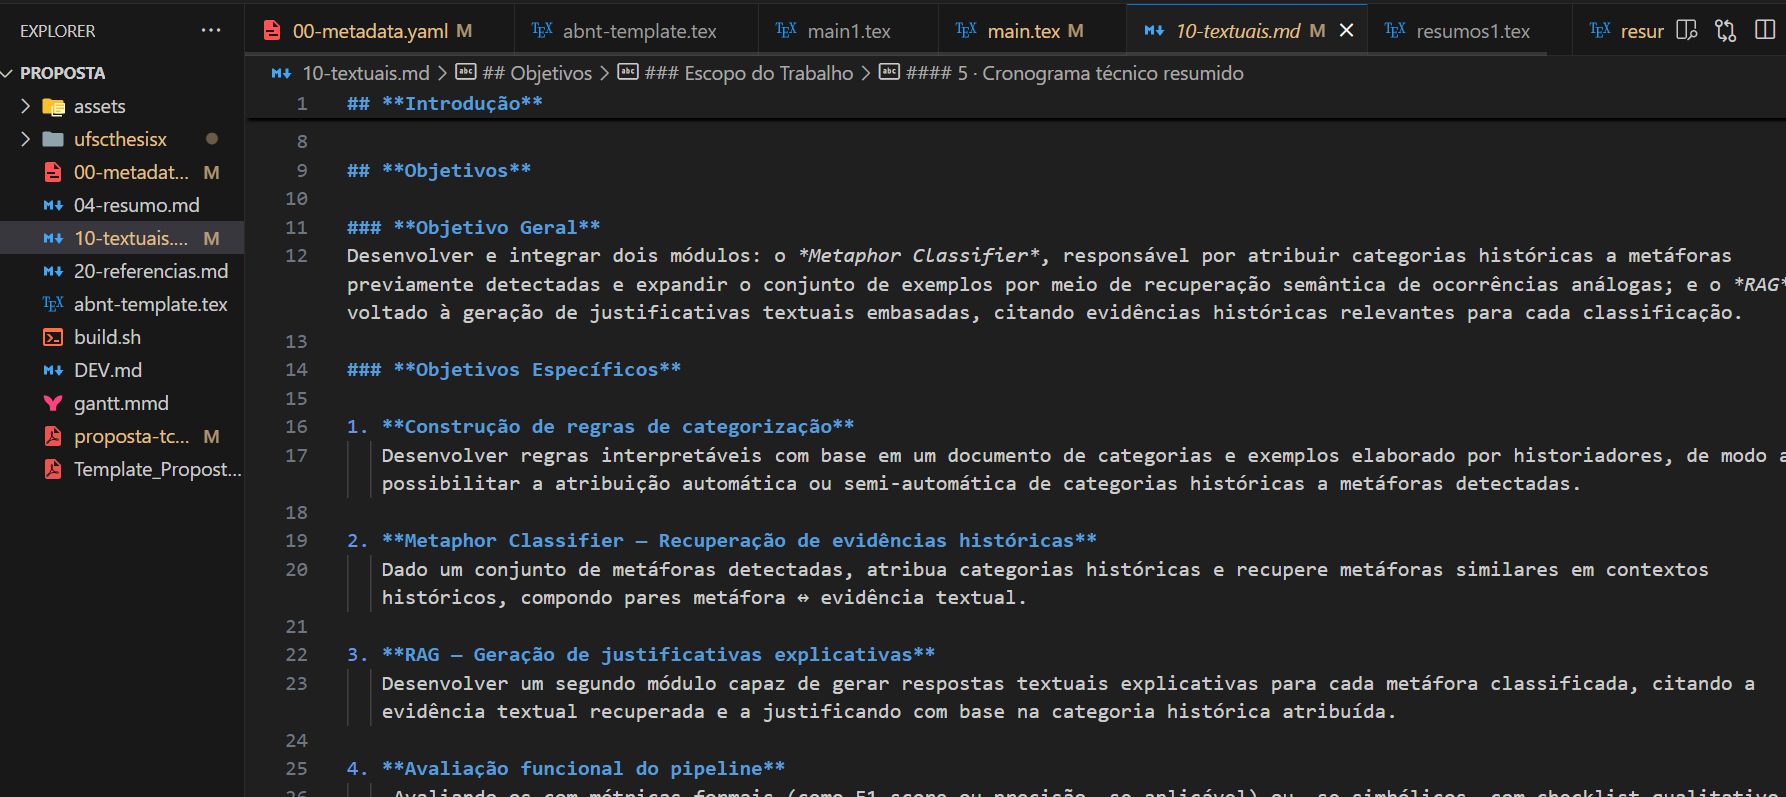
\includegraphics[width=0.6\linewidth]{pictures/intro_topicos.png}
  \caption{Evidência da tarefa US-02A}
\end{figure}

\begin{figure}[htbp]
  \centering
  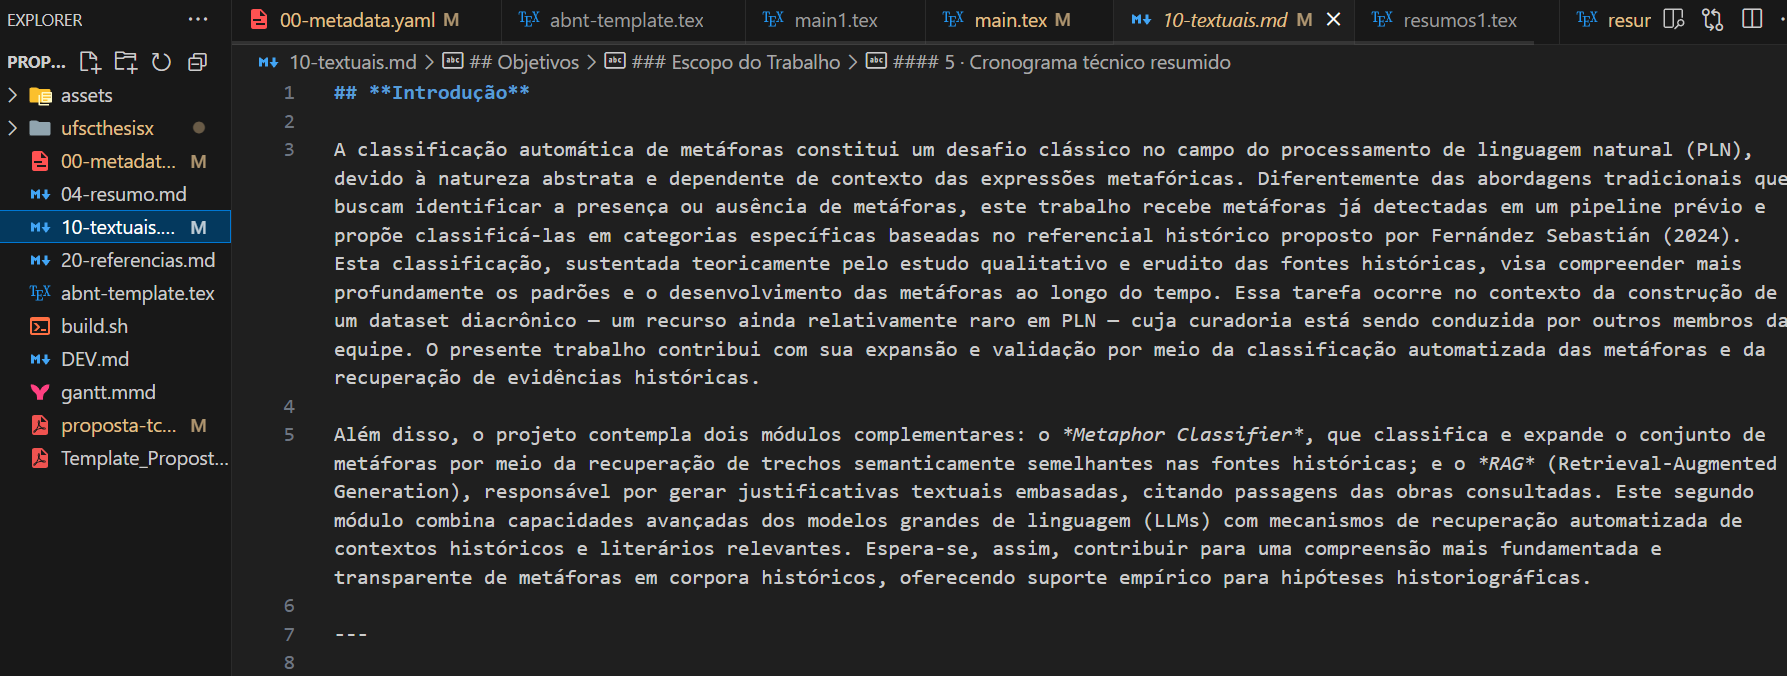
\includegraphics[width=0.6\linewidth]{pictures/intro_rascunho.png}
  \caption{Evidência da tarefa US-02B}
\end{figure}

\begin{figure}[htbp]
  \centering
  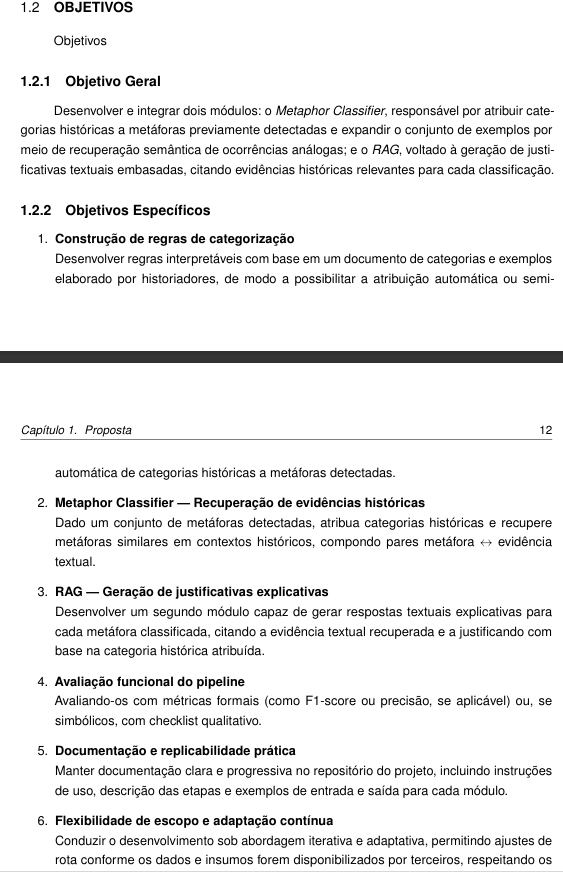
\includegraphics[width=0.6\linewidth]{pictures/problema_objetivos.png}
  \caption{Evidência da tarefa US-03A}
\end{figure}
